\section{Versuchsaufbau}

\begin{figure}[H]
\begin{center}
  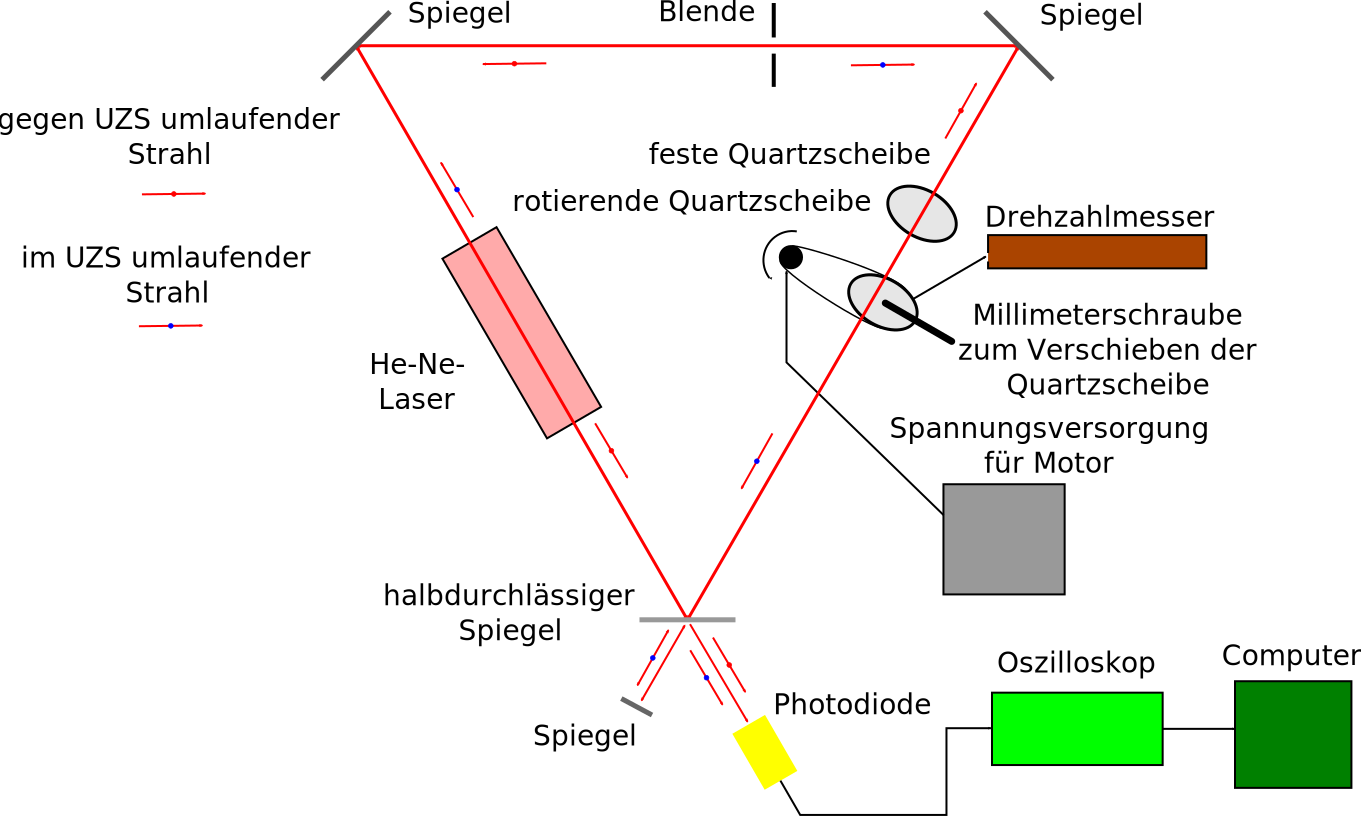
\includegraphics[width=\textwidth]{../img/aufbau.pdf}
  \caption{Versuchsaufbau zur Messung der Kernspinresonanz.}
  \label{img:aufbau}
\end{center}
\end{figure}

\autoref{img:aufbau} zeigt den Aufbau zur Messung der Kernspinresonanz.
Von einem Netzteil wird ein Gleichstrom von mehreren Ampere durch zwei Spulen geschickt,
die durch einen Eisenkern verbunden sind.
Auf dem Eisenkern befinden sich außerdem zwei kleinere Modulationsspulen,
mit denen das hohe statische Magnetfeld noch leicht abgeändert werden kann.
Zwischen den Modulationsspulen ist die zu untersuchenden Probe eingebaut,
die sich in einer weiteren Spule befindet.
Diese Spule und die Modulationsspule werden von einem Netzgerät angesteuert,
an dem Frequenz und Amplitude der Ströme gewählt werden können.
Das Signal an den Modulationsspulen sowie die Amplitude des HF-Signals an der Probenspule
werden von einem Oszilloskop angezeigt.\\
Mit einer Hall-Sonde kann die Stärke des Magnetfelds am Ort der Probe bestimmt werden.